\chapter{Introducción}

Las estrellas son formadas a partir de nubes de gas interestelar, compuestas en su mayoría de hidrógeno molecular, que debido a algún tipo de perturbación comienzan a colapsar gravitacionalmente. La compresión del gas incrementa su temperatura hasta que la presión es capaz de balancearla, alcanzando el equilibrio hidrostático. Este equilibrio dura poco debido a que la pérdida de energía (en forma de radiación) disminuye la temperatura del gas y la consecuente reducción de la presión permite que la contracción continúe. El proceso de contracción y equilibrio del material se repite durante un periodo de tiempo (fase pre-secuencia principal), hasta que la temperatura aumenta lo suficiente para que la fusión de hidrógeno en helio pueda ocurrir en el núcleo ($T\approx 10^7\,\si{\kelvin}$). Este proceso de fusión nuclear compensa las pérdidas radiativas y mantiene a la estrella en un equilibrio hidrostático estable \cite{Scilla2016}.

Las reacciones nucleares pueden sostener a la estrella durante la mayor parte de su vida luminosa (de millones a billones de años, dependiendo de su masa inicial \cite{Salaris2005EvolutionPopulations}). Estrellas en esta fase forman la secuencia principal del diagrama de Hertzsprung-Russell.
\setcounter{footnote}{0}
\begin{figure}[H]
    \centering
    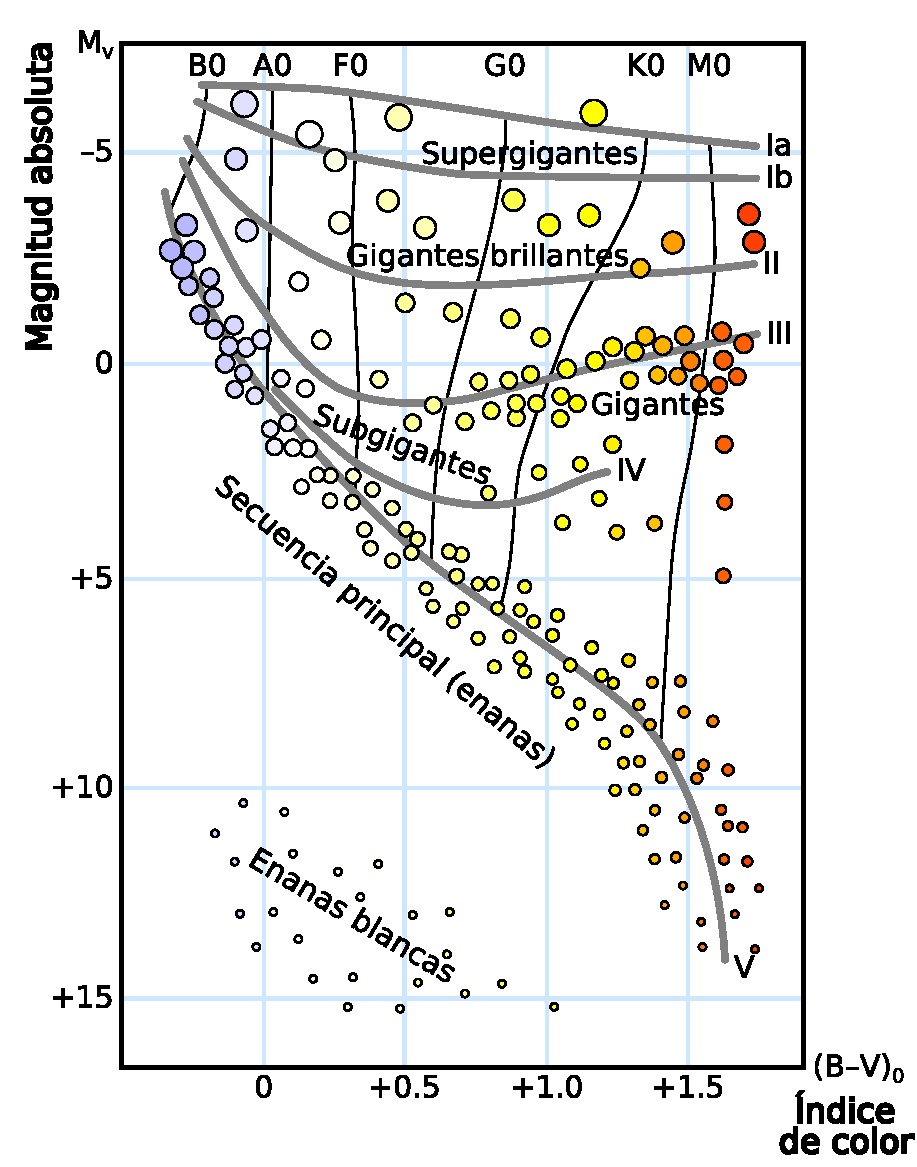
\includegraphics[width=205pt]{figures/H-R_diagram.pdf}%
    \caption[Diagrama Hertzsprung-Russell]{Diagrama Hertzsprung-Russell.\protect\footnotemark}
    \label{HR}
\end{figure}
\footnotetext{Original de \url{https://commons.wikimedia.org/wiki/File:H-R_diagram.svg}}

La evolución de la estrella después de agotar el hidrógeno depende de su masa: estrellas con \emph{masas pequeñas e intermedias} ($M\leq M_{\odot}$) procederán a fusionar helio formando carbono en su núcleo. Esto representa una transición de la secuencia principal hacia la rama de gigantes (hacia el rojo) en el diagrama de Hertzsprung-Russell. Durante las últimas etapas de evolución, estas estrellas liberan sus capas más externas formando una nebulosa planetaria y dejando un núcleo que será sostenido por la presión de degeneración de electrones, conocido como una enana blanca \cite{Padmanabhan2000}.

Estrellas \emph{masivas} ($M>8 M_{\odot}$) entran en un ciclo de fusión de elementos en su núcleo, formando elementos cada vez más pesados (helio, carbono, oxígeno, magnesio, silicio y hierro) \cite{Glendenning2000}. Al final de cada una de estas etapas de fusión los elementos pesados recién creados formarán un núcleo, y los restos del elemento ligero forman un cascarón a su alrededor. En el diagrama de Hertzsprung-Rusell estas estrellas llegarán hasta la parte superior de la secuencia principal y se moverán hacia la rama de supergigantes. Al alcanzar el hierro, la fusión deja de ser exotérmica (en vez de liberar energía la requerirá) y deja a la estrella sin una fuente de energía que mantenga el equilibrio hidrostático. Estas estrellas colapsarán eventualmente en un evento conocido como supernova (tipo II)\cmmt{ de colapso de núcleo}: los cascarones de los distintos elementos caen sobre el núcleo de hierro desencadenando, mediante mecanismos que no han sido enteramente comprendidos \cite{Janka2012}, la eyección de gran parte de su masa en una explosión \cite{Woosley2005}.

Tras la supernova, el núcleo colapsado \cmmt{ —cuya composición precisa no se conoce pero se presume contiene neutrones, protones, mesones, hiperones e incluso quarks desconfinados—}  inicia un proceso de enfriamiento y reajuste estructural, durante el cual emite una gran cantidad de energía en forma de radiación y neutrinos (importantes a la hora de verificar modelos teóricos, cf. \cite{Alvarez-Salazar2018AboutEmission}). Después de alcanzar una composición estable —no conocida con precisión pero se presume contiene neutrones, protones, mesones, hiperones e incluso quarks desconfinados \cite{Lattimer2004}— la presión de degeneración de sus componentes y la repulsión de rango corto entre nucleones sostendrán el núcleo colapsado \cite{Glendenning2000}, alcanzando una estructura definida conocida generalmente como un objeto compacto o estrella de neutrones.
En estos objetos se pueden alcanzar densidades superiores a la densidad de saturación nuclear ($\rho_0 = \num{2.3e+14}\,\si{\g/cm^3}$) y potenciales gravitacionales altos ($\num{1.8e+20}\,\rm{erg/g}$) donde la Relatividad General es importante para determinar su estructura. El comportamiento preciso de la materia nuclear en condiciones tan extremas es desconocido, debido a esto, las estrellas de neutrones son laboratorios de materia nuclear ultradensa y se han convertido en un tema de interés en el campo de la astrofísica nuclear.

El trabajo de grado tendrá como objetivo obtener modelos de objetos compactos en equilibrio, usando ecuaciones de estado que describan distintas composiciones de materia ultradensa y que cumplan con ciertas condiciones de aceptabilidad física. \cmmt{y mediante algunas condiciones de aceptabilidad física identificar modelos que sean de interés astrofísico.}

Esta propuesta está organizada de la siguiente manera: en el marco teórico se presentarán los elementos básicos de estructura estelar newtoniana y relativista; una discusión sobre la estructura interior y la ecuación de estado de estrellas de neutrones y una recopilación de condiciones de aceptabilidad física para modelos estelares. Posteriormente se identificarán los objetivos del trabajo de grado y se presentará una metodología mediante la cual se pretende cumplir estos objetivos.
%\begin{multicols}{2}[\columnsep2em] 

%\columnbreak
%\end{multicols}  
%y resultarán, después de un evento complejo y violento, como una estrella de neutrones o un agujero negro. \REMARK{No he hablado ni de estrellas de neutrones ni de agujeros negros...} 
